\part{Ranklust}
\label{pa:ranklust}
\chapter{Workflow and usage}
\section{For researchers}
The way researchers will work with Ranklust is pretty simple. Step 1 and 2 will
only be required the first time the researcher want to use this app to solve
his/her problem. The rest has to be done every time, unless a previous session
of Cytoscape is loaded with more developed results.

\begin{enumerate}
    \item Install Cytoscape
    \item Install clusterMaker2 plugin through Cytoscape App manager
    \item Upload the network to be clustered and ranked into Cytoscape
    \item Use clusterMaker2 to cluster the network
    \item Use the Ranklust-part of clusterMaker2 to rank the clusters
        \begin{enumerate}
            \item Decide what to score the clusters on
        \end{enumerate}
    \item Use the Ranklust-part of clusterMaker2 to visualize the rankings
\end{enumerate}

Step 6 should show the researchers the ranking of clusters based on what
attributes they wanted to include in step 5a. This ranking represents cluster
biomarkers. The score of the clusters and the order they are ranked in will
decide the state of the patient. State of the patient can be many different
things and what the rankings will mean to the researcher is not yet final. It
will be a new indicator, a biomarker, and information about what it means has to
be gathered empirically through clinical research.

\section{Workflow image examples}
\begin{figure}[h]
    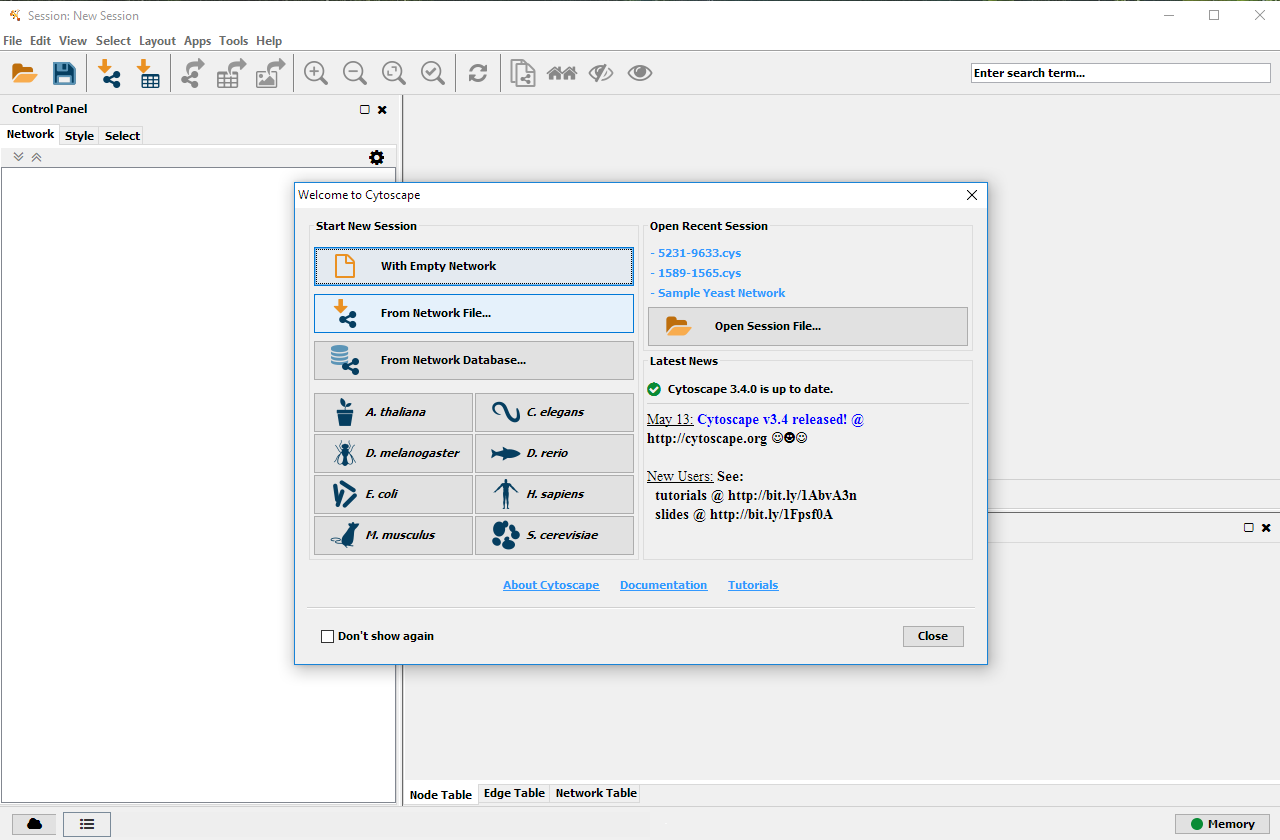
\includegraphics[width=15cm]{1-startup}
\end{figure}
\begin{figure}[h]
    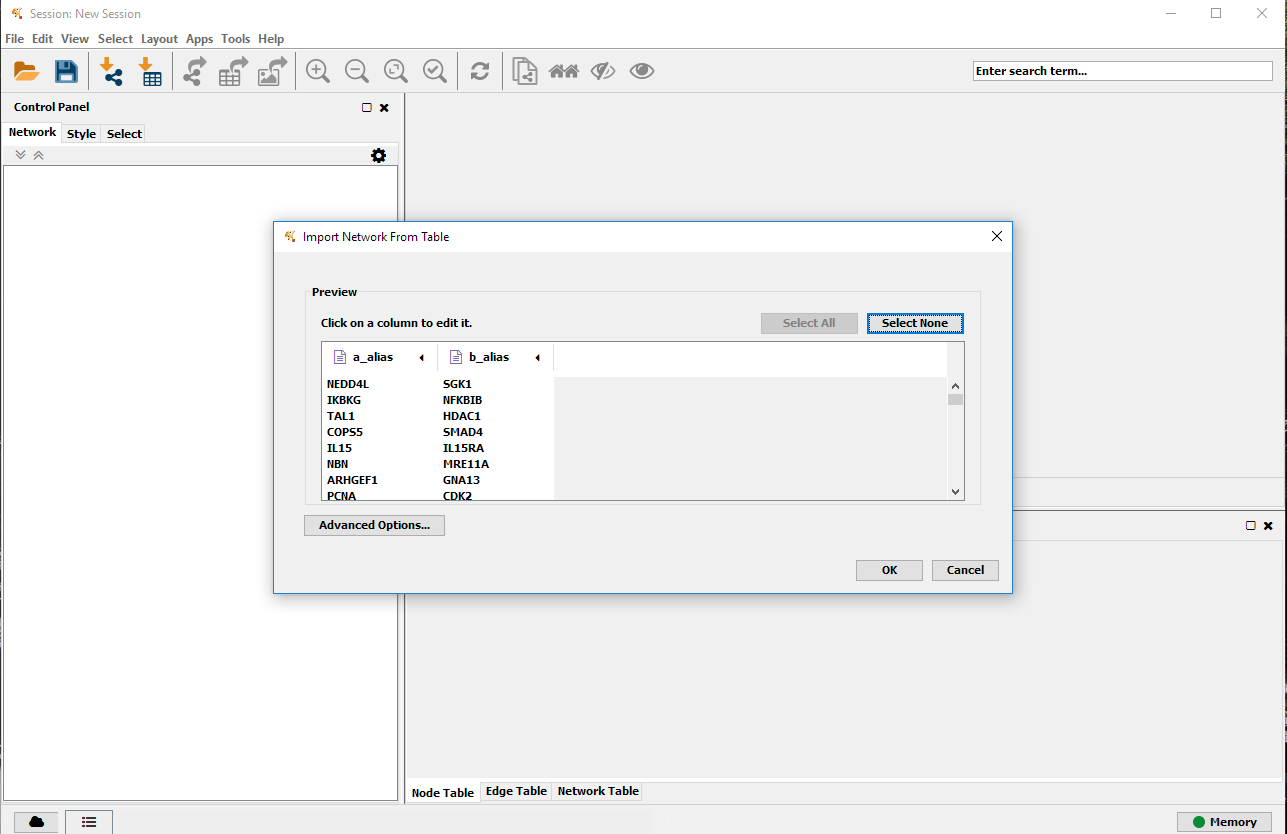
\includegraphics[width=15cm]{2-import}
\end{figure}
\begin{figure}[h]
    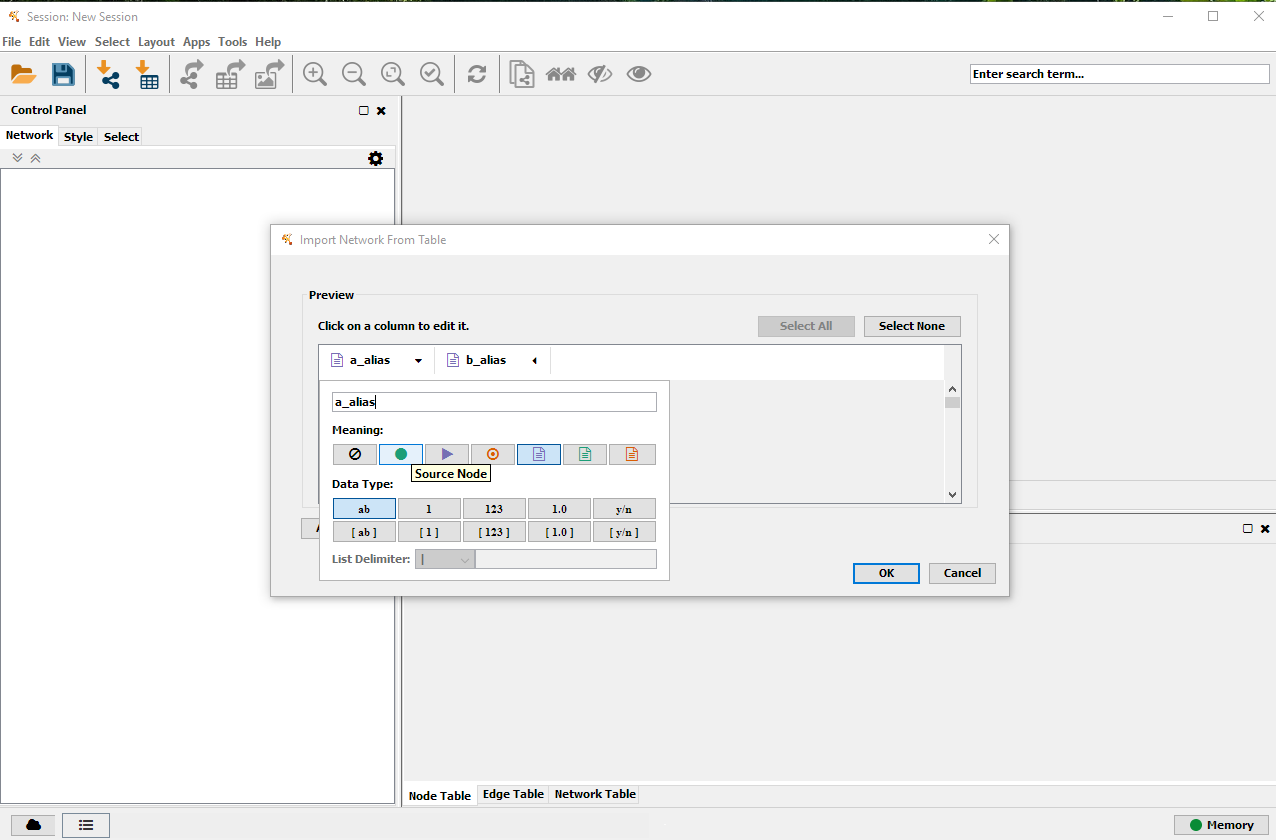
\includegraphics[width=15cm]{3-nodes}
\end{figure}
\begin{figure}[h]
    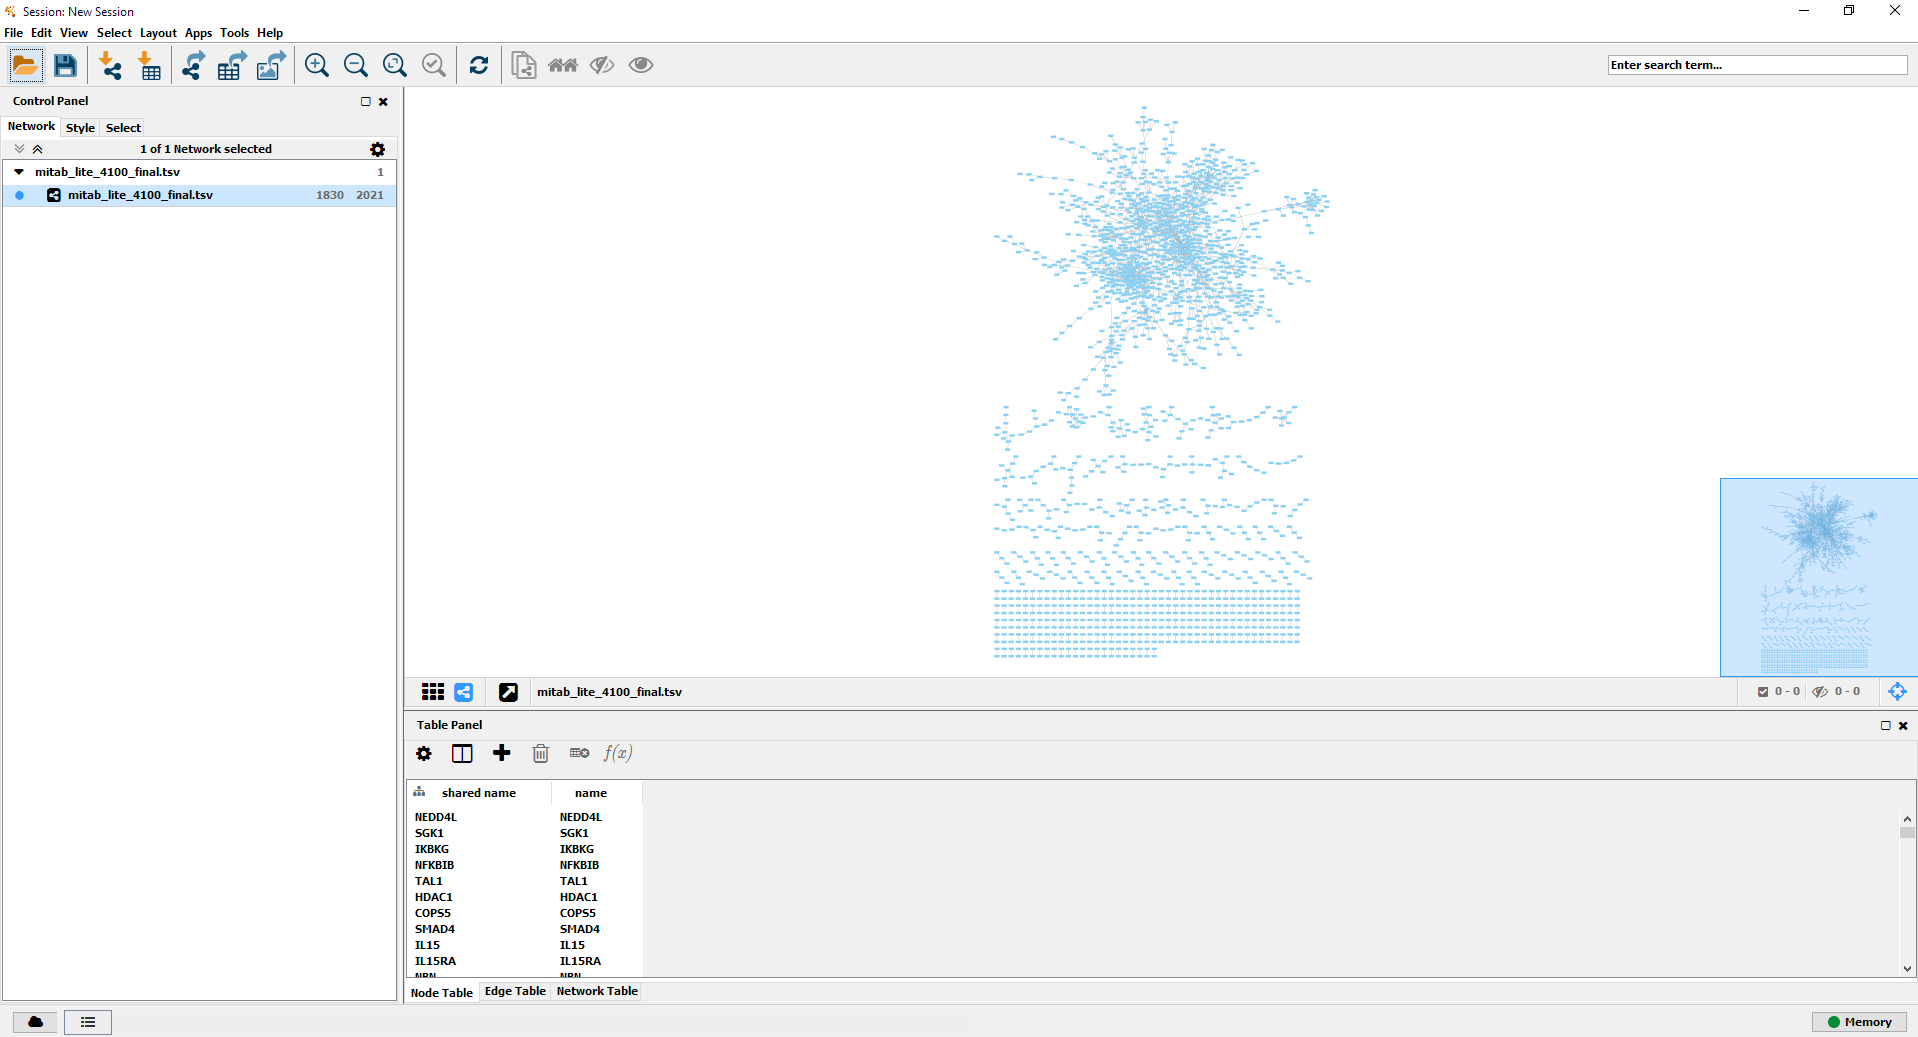
\includegraphics[width=15cm]{4-imported-network}
\end{figure}
\begin{figure}[h]
    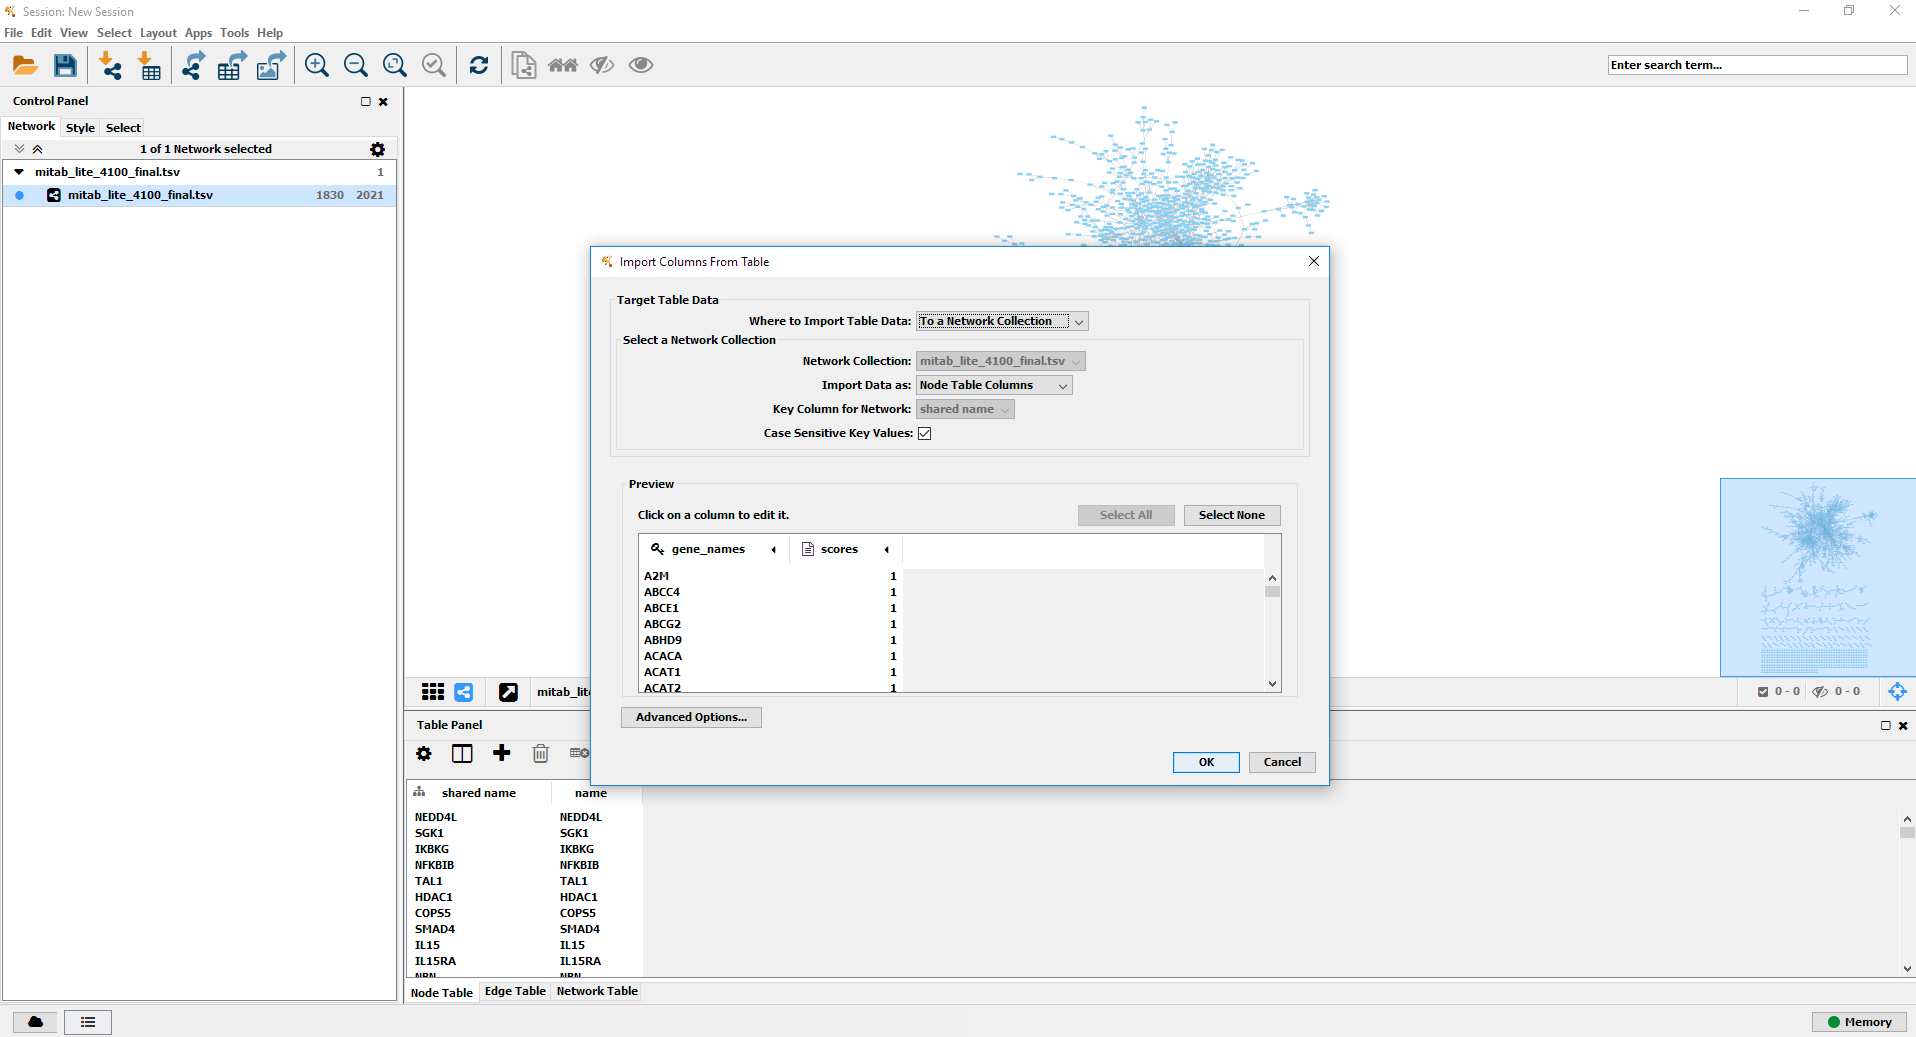
\includegraphics[width=15cm]{5-import-table}
\end{figure}
\begin{figure}[h]
    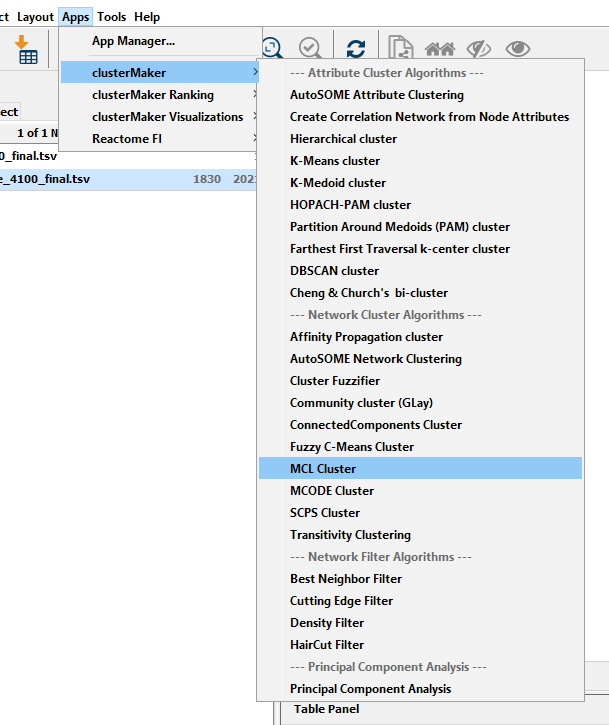
\includegraphics[width=15cm]{6-cluster}
\end{figure}
\begin{figure}[h]
    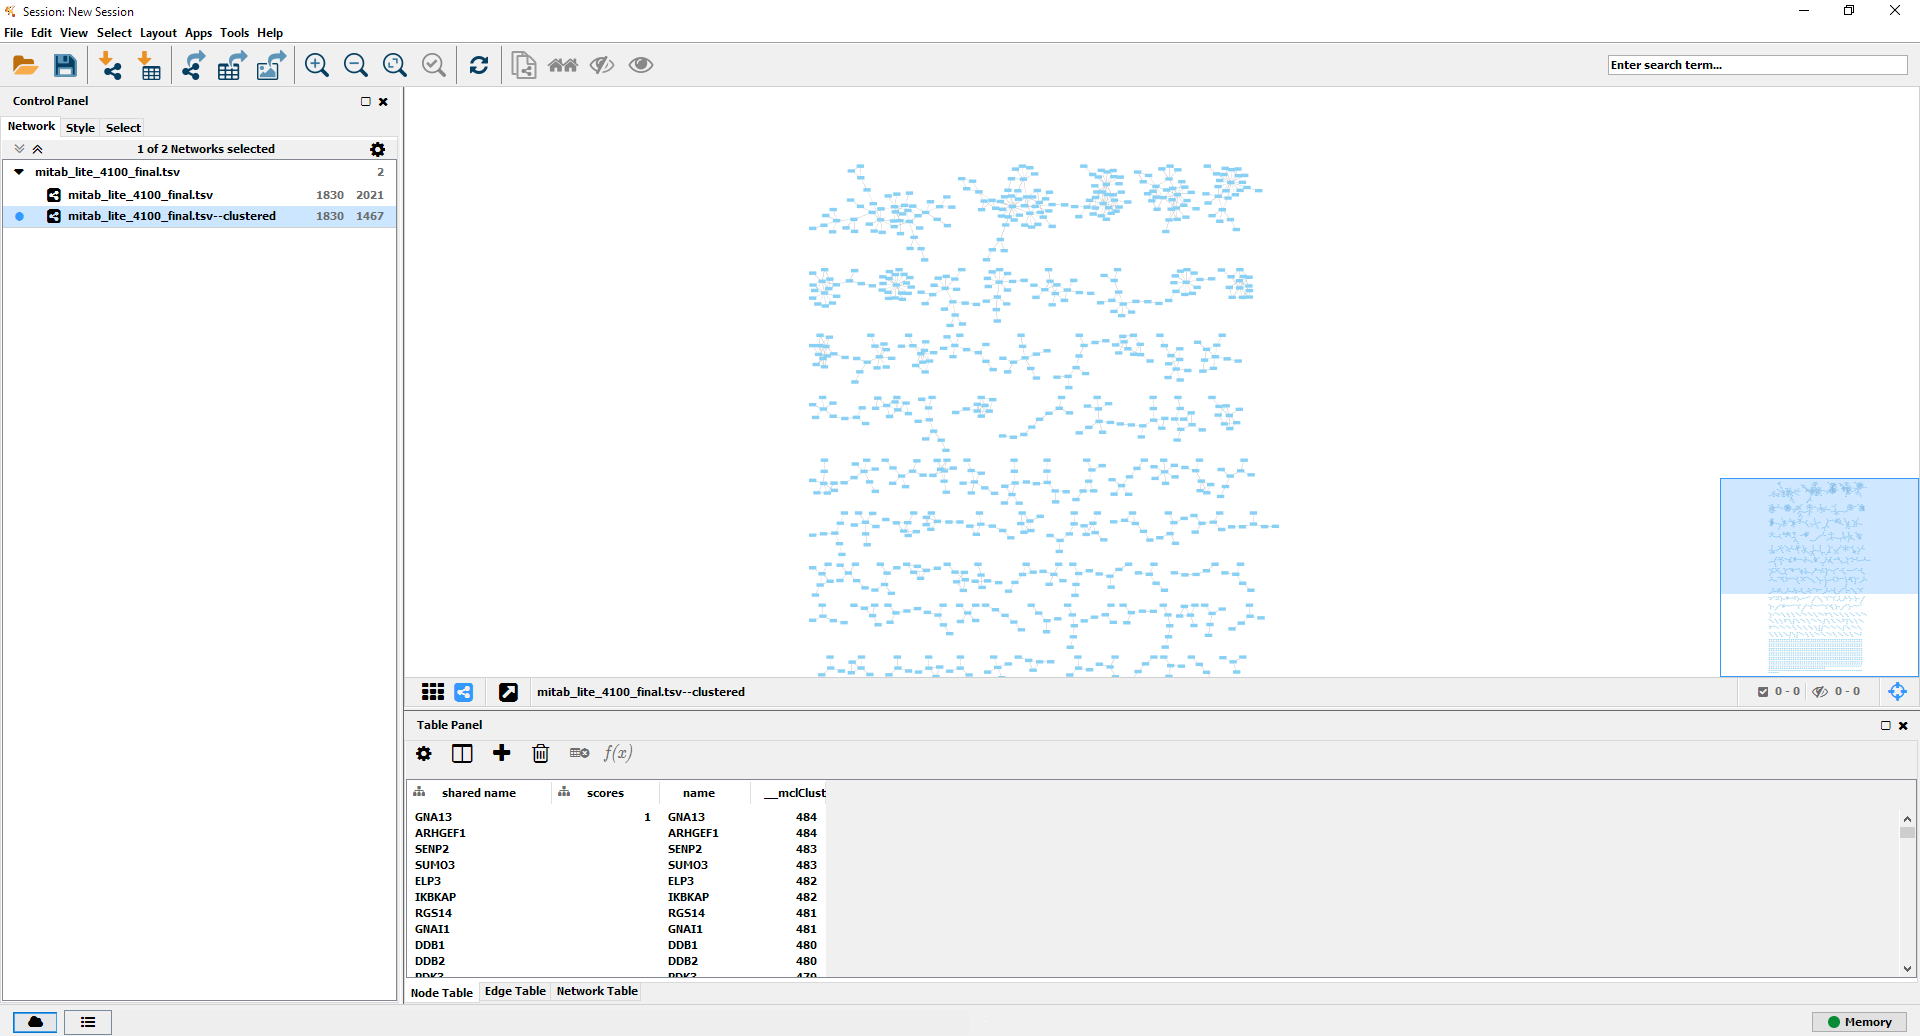
\includegraphics[width=15cm]{7-done-cluster}
\end{figure}
\begin{figure}[h]
    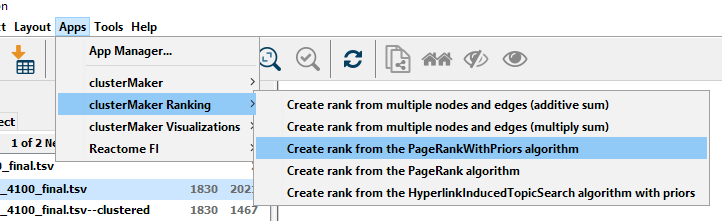
\includegraphics[width=15cm]{8-choose-ranking}
\end{figure}
\begin{figure}[h]
    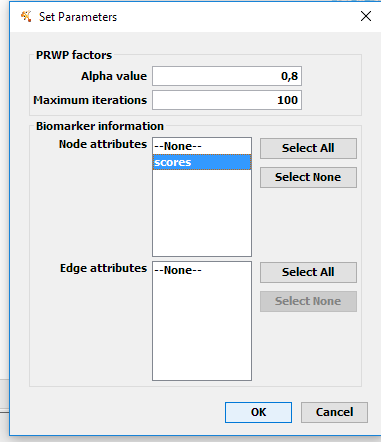
\includegraphics[width=15cm]{9-pagerank}
\end{figure}
\begin{figure}[h]
    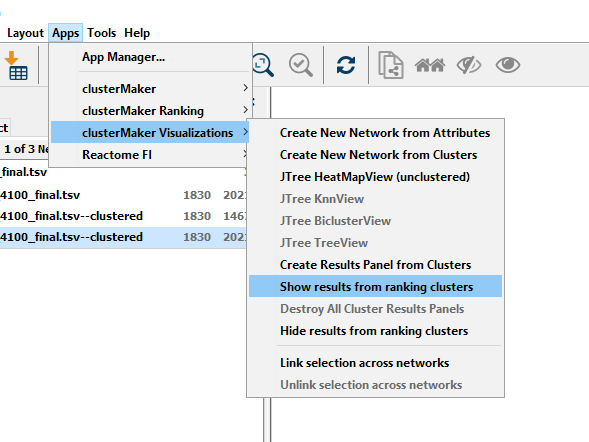
\includegraphics[width=15cm]{10-show-results}
\end{figure}
\begin{figure}[h]
    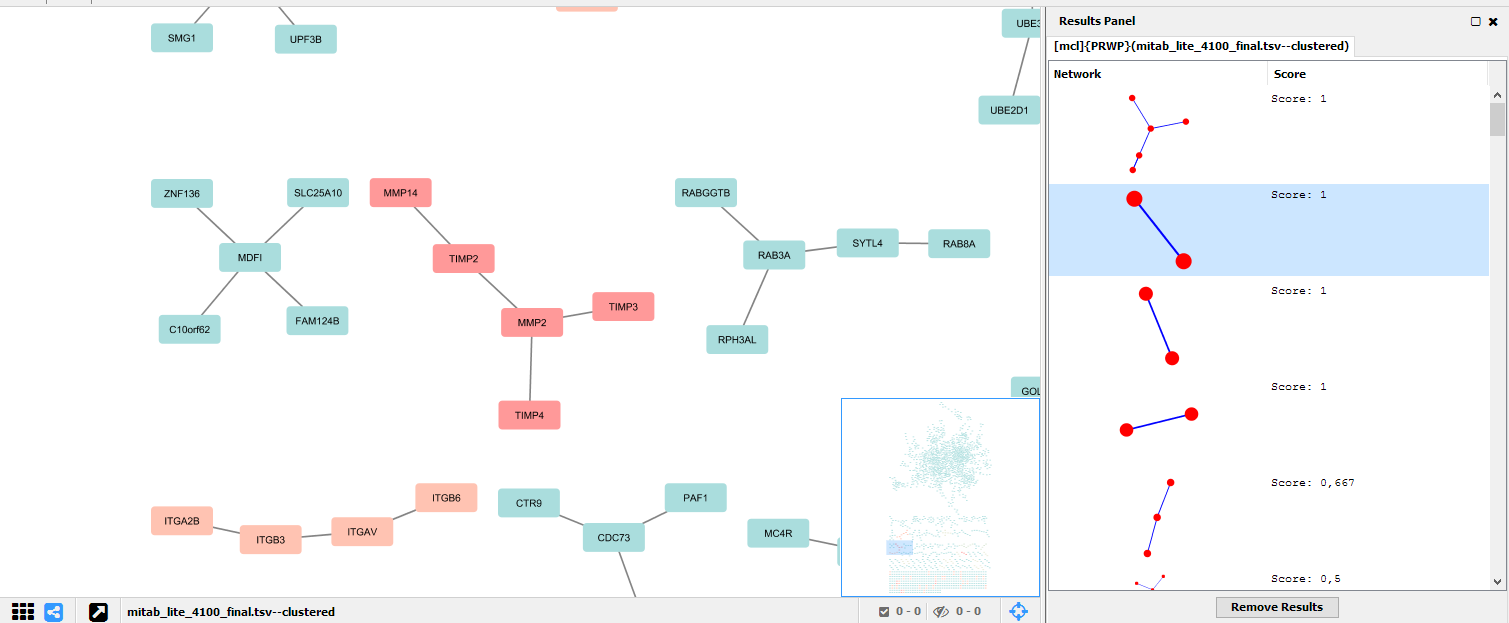
\includegraphics[width=15cm]{11-result-colors}
\end{figure}
\begin{figure}[h]
    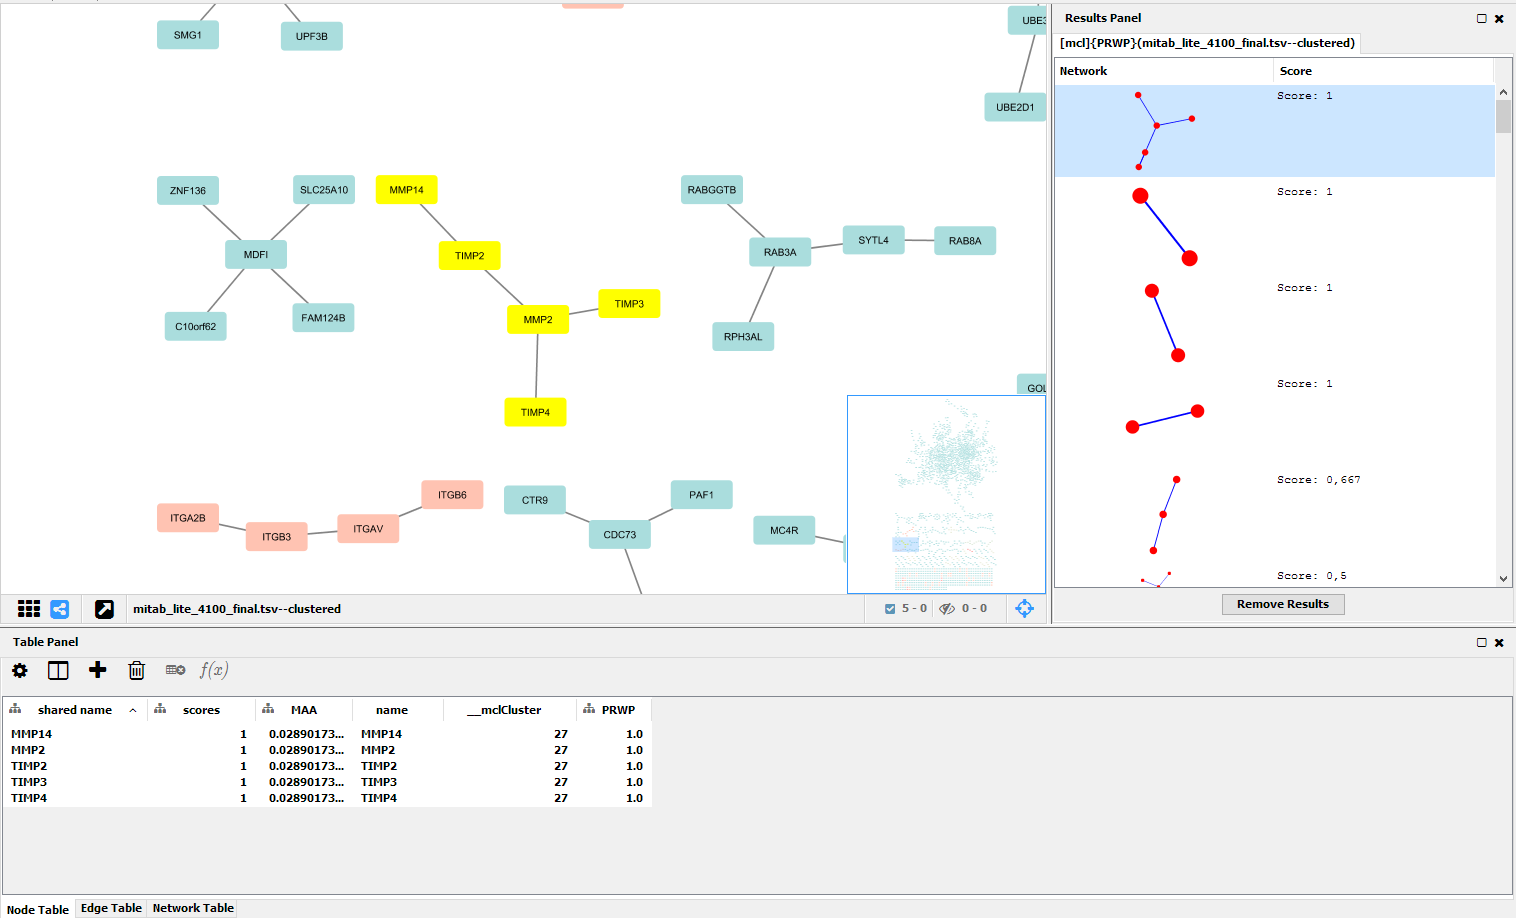
\includegraphics[width=15cm]{12-rank-selection}
\end{figure}
